\documentclass[11pt,a4paper]{article}

% --- Essential Packages ---
\usepackage[utf8]{inputenc}
\usepackage{geometry}
\geometry{
  a4paper,
  top=1in,
  bottom=1in,
  left=1in,
  right=1in
}
\usepackage{amsmath,amssymb}
\usepackage{graphicx}
\usepackage{tabularx}
\usepackage{booktabs}
\usepackage{cite}
\usepackage{enumitem}
\usepackage{float}
\usepackage{titlesec}
\usepackage{tikz}
\usetikzlibrary{shapes.geometric, arrows.meta, positioning, calc}
\usepackage[none]{hyphenat}
\usepackage{setspace}
\onehalfspacing

% --- Hyperlink Setup ---
\usepackage{hyperref}
\hypersetup{
    colorlinks=true,
    linkcolor=blue,
    filecolor=magenta,      
    urlcolor=cyan,
    citecolor=blue,
}

% --- Document Metadata ---
\title{\textbf{DarkSight: A Real-Time, Client-Side Framework for Multi-Modal Dark Pattern Detection and Dynamic Countermeasures}}
\author{
    \textbf{Miftahul Islam Tashfin}, \textbf{Nipu Basher}, \textbf{Mahbubur Rahman Ovi}, \textbf{Muntasir Ahmed Rifat} \\[0.5em]
    \small Department of Computer Science and Engineering, East West University \\
    \small \texttt{\{tashfin, basher, ovi, rifat\}@ewubd.edu}
}
\date{\today}

\begin{document}

\maketitle

% --- Abstract ---
\begin{abstract}
\noindent Dark patterns are deceptive user interface (UI) architectures engineered to subconsciously manipulate users into unintended actions such as impulse purchases, hidden recurring subscriptions, or privacy concessions. While extensive academic literature has focused on taxonomy definition and offline dataset classification, existing detection tools do not actively neutralize deceptive patterns in real time or require transmitting private browsing data to remote servers. In this paper, we propose \textbf{DarkSight}, a novel, privacy-preserving browser extension that combines six foundational detection frameworks and one dynamic countermeasure framework into an asynchronous, client-side runtime. DarkSight features a multi-tiered cascade: Tier-1 zero-latency regex heuristics for explicit linguistic patterns, Tier-2 semantic reasoning powered by a local DeepSeek-R1 Large Language Model (LLM), Tier-3a structural CSS geometry analysis for false visual hierarchies (AidUI), and Tier-3b spatial multimodal vision scanning (Qwen2.5-VL via DP Sentinel). Beyond passive detection, DarkSight introduces an active Countermeasure Dispatcher that transforms flagged elements in-situ through Highlight \& Explain (HLE), Hide (HD), and Switch (SW) transformations. Empirical evaluations against benchmark datasets and live e-commerce websites demonstrate a 70.07\% textual detection accuracy and an 80.73\% visual detection accuracy, effectively establishing a practical paradigm for real-time consumer defense on the modern web.
\end{abstract}

\vspace{1em}
\noindent \textbf{Keywords:} Dark Patterns, Deceptive UI, Browser Extension, Client-Side LLM, Multimodal Vision, Real-Time Countermeasures, AidUI, DP Sentinel.

\vspace{2em}

% ==============================================================================
% 3. METHODOLOGY
% ==============================================================================
\section{Methodology}
\label{sec:methodology}

\subsection{Overview and System Architecture}
\label{subsec:overview_arch}

Most existing literature on dark patterns examines only an isolated slice of the manipulation spectrum. Prior works typically analyze textual cues, parse DOM trees, or audit rendered screenshots retroactively on offline datasets long after user interaction has concluded \cite{mathur2019, schaefer2023, aidui2023, 50shades, dpsentinel2024}. While these studies provide foundational taxonomies, they leave a critical operational void: none simultaneously detect dark patterns \textit{and} neutralize them in real time within the active browser session, and none do so without transmitting sensitive user browsing telemetry to external cloud servers.

DarkSight addresses this limitation by uniting six established detection frameworks and one dynamic countermeasure model into a unified, privacy-first, client-side browser runtime. The system orchestrates lightweight regex pattern matching, structural CSS calculations, semantic language reasoning, and multimodal spatial computer vision into an asynchronous, tiered cascade. Crucially, detection does not terminate in passive analytical reporting. Every confirmed signal is routed to an autonomous countermeasure engine that applies live UI interventions directly on the active webpage \cite{schaefer2024}.

% --- Architecture Diagram Placeholder (Compiles out-of-the-box on Overleaf) ---
\begin{figure*}[htbp]
    \centering
    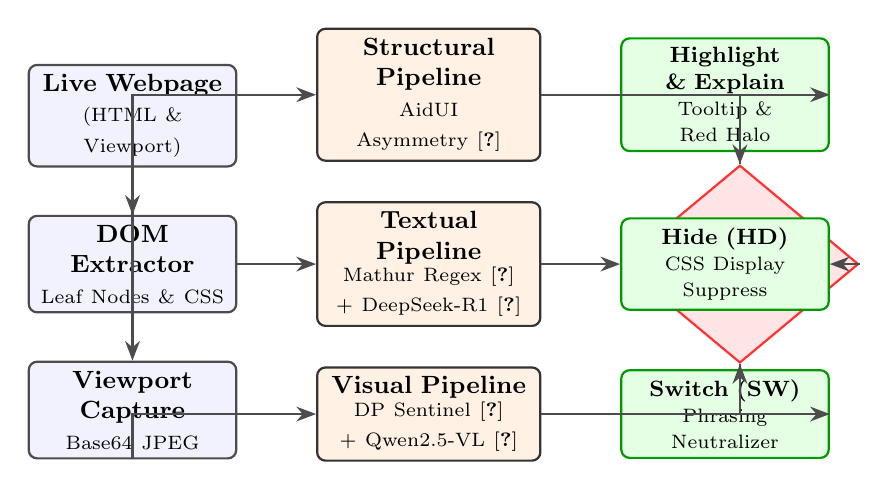
\begin{tikzpicture}[
        node distance=0.8cm and 0.8cm,
        box/.style={rectangle, draw=black!70, thick, fill=blue!5, rounded corners=3pt, text width=2.4cm, minimum height=1.1cm, align=center, font=\small},
        proc/.style={rectangle, draw=black!80, thick, fill=orange!10, rounded corners=3pt, text width=2.6cm, minimum height=1.1cm, align=center, font=\small},
        disp/.style={diamond, draw=red!80, thick, fill=red!10, text width=1.8cm, minimum height=1.6cm, align=center, font=\footnotesize, aspect=1.2},
        action/.style={rectangle, draw=green!60!black, thick, fill=green!10, rounded corners=3pt, text width=2.4cm, minimum height=0.9cm, align=center, font=\footnotesize},
        arrow/.style={-{Stealth[length=2.5mm]}, thick, draw=black!70}
    ]
        % Column 1: Ingestion
        \node[box] (webpage) {\textbf{Live Webpage}\\\scriptsize (HTML \& Viewport)};
        \node[box, below=0.6cm of webpage] (dom) {\textbf{DOM Extractor}\\\scriptsize Leaf Nodes \& CSS};
        \node[box, below=0.6cm of dom] (vport) {\textbf{Viewport Capture}\\\scriptsize Base64 JPEG};

        % Column 2: Pipelines
        \node[proc, right=1.0cm of dom] (textpipe) {\textbf{Textual Pipeline}\\\scriptsize Mathur Regex \cite{mathur2019}\\+ DeepSeek-R1 \cite{schaefer2023}};
        \node[proc, above=0.5cm of textpipe] (aidui) {\textbf{Structural Pipeline}\\\scriptsize AidUI Asymmetry \cite{aidui2023}};
        \node[proc, below=0.5cm of textpipe] (vision) {\textbf{Visual Pipeline}\\\scriptsize DP Sentinel \cite{dpsentinel2024}\\+ Qwen2.5-VL \cite{50shades}};

        % Column 3: Dispatcher
        \node[disp, right=1.0cm of textpipe] (dispatch) {\textbf{Strategy}\\ \textbf{Dispatcher}};

        % Column 4: Interventions
        \node[action, right=1.0cm of aidui] (hle) {\textbf{Highlight \& Explain}\\\scriptsize Tooltip \& Red Halo};
        \node[action, right=1.0cm of textpipe] (hd) {\textbf{Hide (HD)}\\\scriptsize CSS Display Suppress};
        \node[action, right=1.0cm of vision] (sw) {\textbf{Switch (SW)}\\\scriptsize Phrasing Neutralizer};

        % Arrows
        \draw[arrow] (webpage) -- (dom);
        \draw[arrow] (webpage) -- (vport);
        \draw[arrow] (dom) |- (aidui);
        \draw[arrow] (dom) -- (textpipe);
        \draw[arrow] (vport) |- (vision);

        \draw[arrow] (aidui) -| (dispatch);
        \draw[arrow] (textpipe) -- (dispatch);
        \draw[arrow] (vision) -| (dispatch);

        \draw[arrow] (dispatch) |- (hle);
        \draw[arrow] (dispatch) -- (hd);
        \draw[arrow] (dispatch) |- (sw);
    \end{tikzpicture}
    \caption{The end-to-end architecture of DarkSight, illustrating the dual ingestion pipeline, three-tiered detection cascade, and the runtime countermeasure dispatcher.}
    \label{fig:full_arch}
\end{figure*}

\subsubsection{Detailed Left-to-Right Architectural Walkthrough}
\label{subsubsec:arch_walkthrough}

Reading Figure~\ref{fig:full_arch} from left to right demonstrates how raw web content is ingested, evaluated across three specialized pipelines, and transformed into defensive UI mitigations:

\begin{enumerate}[leftmargin=*]
    \item \textbf{Dual-Stream Data Ingestion (Left):} When a webpage loads, DarkSight's content script initiates two concurrent data capture streams:
    \begin{itemize}
        \item \textit{DOM Leaf-Node \& Style Extraction:} Recursively traverses the live HTML DOM tree to isolate raw textual strings while capturing computed CSS bounding box geometry and color values (\texttt{window.getComputedStyle}) from interactive components.
        \item \textit{Viewport Snapshot Capture:} Simultaneously, the background service worker invokes \texttt{chrome.tabs.captureVisibleTab} to serialize the visible viewport into a high-resolution, Base64-encoded image stream.
    \end{itemize}

    \item \textbf{Tri-Pipeline Detection Cascade (Center):} The ingested data splits across three complementary detection engines operating at different abstraction levels:
    \begin{itemize}
        \item \textit{Textual Pipeline (Tier 1 \& Tier 2):} Ingested text strings are first evaluated by a zero-latency Fast Regex Engine to intercept explicit urgency and scarcity triggers. Ambiguous phrases bypass regex and are passed asynchronously to a local DeepSeek-R1 Large Language Model (LLM) via Ollama, utilizing Chain-of-Thought (CoT) semantic reasoning to identify subtle psychological manipulation.
        \item \textit{Structural Pipeline (Tier 3a):} Sibling interactive elements (e.g., ``Accept'' vs. ``Decline'' buttons) enter the AidUI Structural Engine, which calculates surface area and color contrast ratios to expose false visual hierarchies.
        \item \textit{Visual Multimodal Pipeline (Tier 3b):} The graphical viewport screenshot is streamed directly to a local Qwen2.5-VL multimodal vision model, mapping 21 visual deception categories and predicting exact spatial bounding boxes for elements that evade the DOM.
    \end{itemize}

    \item \textbf{Strategy Dispatcher (Right-Center):} Flags emitted by any of the three detection pipelines converge at DarkSight's central arbitration core: the Countermeasure Dispatcher. The dispatcher resolves the target DOM node (or maps visual coordinates back to client-screen pixels) and references the user's active protection profile.

    \item \textbf{Live DOM Interventions (Far Right):} The DOM Transformer executes client-side mutations on the live webpage: wrapping the manipulative node in an explanatory halo (\textbf{Highlight \& Explain}), visually collapsing the element (\textbf{Hide}), or rewriting deceptive phrasing into neutral text (\textbf{Switch}).
\end{enumerate}

% ------------------------------------------------------------------------------
\subsection{Dual Data Ingestion: DOM Extraction and Viewport Capture}
\label{subsec:ingestion}

Real-time browser intervention requires capturing both the underlying code structure and the rendered visual state. DarkSight executes this through a dual-stream ingestion pipeline that decouples textual and structural metadata from graphical page rendering.

The \textbf{DOM Extractor} operates inside an isolated content script (\texttt{content.js}). Rather than passing the entire uncurated HTML document to downstream models—which introduces prohibitive token overhead and processing delay—it recursively traverses the document tree to extract visible leaf nodes. For every text node and interactive container (\texttt{<button>}, \texttt{<a>}, \texttt{<input>}), the extractor strips irrelevant attributes, filters out script/style blocks, and computes real-time styling parameters using \texttt{window.getComputedStyle()}. This packages every candidate element with its raw text, foreground color, background color, font size, and rendered bounding box coordinates (\texttt{getBoundingClientRect()}).

Concurrently, the \textbf{Viewport Capture Engine} accesses Chrome's extension API (\texttt{chrome.tabs.captureVisibleTab}) from the service worker (\texttt{background.js}). Triggered with a single-execution guard after page load, it takes a clean visual snapshot of the rendered screen. This dual ingestion architecture ensures that text-based heuristics operate with near-zero latency, while visual analysis retains full contextual awareness of graphical tricks like disguised ads, deceptive countdown clocks, or invisible dismissal icons.

% ------------------------------------------------------------------------------
\subsection{The Three Detection Pipelines}
\label{subsec:detection_pipelines}

Dark patterns operate across multiple modalities: some are purely linguistic, some exploit visual contrast, and others hide within overall page layout. DarkSight deploys three specialized pipelines, each built upon established academic research, to cover every vector.

\subsubsection{Textual Pipeline: Tier-1 Heuristics and Tier-2 Semantic Reasoning}
\label{subsubsec:textual_pipeline}

Textual deception relies on manipulative phrasing, false countdown timers, and artificial urgency. DarkSight evaluates text through a two-tiered hybrid cascade that balances execution speed with linguistic depth.

\begin{itemize}[leftmargin=*]
    \item \textbf{Tier 1 (Fast Heuristic Regex Engine):} As the initial line of defense, candidate strings are scanned against an optimized regular expression suite derived directly from the empirical crawl findings of Mathur et al.~\cite{mathur2019}. Mathur's analysis of 11,000 shopping websites revealed that high-pressure text often follows strict syntactic formulations. Our regex engine matches explicit patterns across four baseline categories: \textit{Urgency} (e.g., \texttt{offer expires in}, \texttt{limited time}), \textit{Scarcity} (e.g., \texttt{only \textbackslash d+ left in stock}), \textit{Social Proof} (e.g., \texttt{\textbackslash d+ people viewing right now}), and \textit{Fake Discounts}. Because regex matches execute synchronously in microseconds, obvious manipulative cues are intercepted immediately without touching an AI model.

    \item \textbf{Tier 2 (Semantic LLM Reasoning):} Ambiguous strings that evade regex patterns—such as subtle confirmshaming, passive-aggressive guilt, or convoluted subscription traps—are dispatched to a local DeepSeek-R1 (1.5B) language model. To structure the model's reasoning, we integrate two complementary methodologies:
    \begin{enumerate}
        \item \textit{Schaefer (2023) Taxonomy:} The model's classification space is formally bounded by Schaefer's 8-category textual dark pattern taxonomy (\textit{Urgency, Scarcity, Social Proof, Obstruction, Forced Action, Sneaking, Misdirection, and Fake Discount})~\cite{schaefer2023}.
        \item \textit{In-Context Learning (2023) Methodology:} Following few-shot in-context learning principles~\cite{incontext2023}, the LLM prompt (\texttt{prompt.js}) is constructed with explicit operational definitions, contextual counter-examples, and Chain-of-Thought (CoT) reasoning paths. By demonstrating how to distinguish authentic inventory notices (e.g., ``Event dates: May 26 -- June 2'') from artificial pressure (e.g., ``FLASH SALE ends in 2 hours''), the prompt prevents hallucination and enforces strict classification boundaries during zero-shot runtime inference.
    \end{enumerate}
\end{itemize}

\subsubsection{Structural Pipeline: DOM Geometry and Asymmetry Calculation}
\label{subsubsec:structural_pipeline}

Not all dark patterns rely on manipulative language; many exploit visual friction and spatial layout to coerce user choices. A common manifestation is \textit{False Hierarchy}, where an ``Accept All'' option is rendered as a prominent, high-contrast button, while the ``Decline'' alternative is suppressed into an almost invisible, low-contrast text link. Pure textual models are inherently blind to such visual discrepancies.

DarkSight addresses this by implementing the algorithmic principles of AidUI~\cite{aidui2023}. The structural pipeline identifies sibling interactive elements within the same container, measures their rendered bounding boxes, and calculates color contrast ratios relative to the underlying surface:
\begin{equation}
    \text{Area Ratio} = \frac{\text{Area}_{\text{Primary}}}{\text{Area}_{\text{Secondary}}}
\end{equation}
\begin{equation}
    \text{Contrast Ratio} = \frac{\text{Contrast}(\text{Primary}, \text{Background})}{\text{Contrast}(\text{Secondary}, \text{Background})}
\end{equation}

We improved upon the original AidUI threshold by calibrating the decision boundary to trigger whenever the combined visual discrepancy meets or exceeds 1.0 ($\text{Discrepancy} \ge 1.0$). This allows the engine to flag deceptive button pairs where visual suppression relies purely on low-contrast opacity, even when button dimensions are identical. Elements identified as false hierarchies are flagged for Misdirection and routed directly to the countermeasure dispatcher.

\subsubsection{Visual Multimodal Pipeline: Spatial Screen Understanding}
\label{subsubsec:visual_pipeline}

Complex web interfaces frequently embed dark patterns within raster images, non-standard canvas objects, or complex multi-layer modal dialogues that lack descriptive DOM tags. To capture these, DarkSight incorporates an end-to-end multimodal computer vision pipeline.

We base our vision architecture on DP Sentinel~\cite{dpsentinel2024}, which proposed utilizing multimodal vision models for real-time interface analysis. DarkSight implements this pipeline using the state-of-the-art Qwen2.5-VL model running locally via Ollama.

The model inspects the viewport snapshot against the comprehensive ``50 Shades of Deceptive Patterns'' taxonomy~\cite{50shades}, targeting 21 distinct visual deceptions (including \textit{Gamification wheels, Hidden Costs, Sneak into Basket, Roach Motel, Disguised Ads, and Deceptive Countdown Badges}). Rather than returning abstract text, the vision model performs spatial reasoning to predict normalized coordinates $[y_{\min}, x_{\min}, y_{\max}, x_{\max}]$ for each detected element. DarkSight maps these normalized coordinates back to the user's active viewport pixel resolution, creating a visible defensive boundary over purely visual traps.

% ------------------------------------------------------------------------------
\subsection{The Countermeasure and Neutralization Engine}
\label{subsec:countermeasures}

The pipelines described above address detection—which is precisely where existing academic literature stops. Across the source papers we build upon, contributions end at dataset classification, precision benchmarking, or offline reporting. DarkSight's primary practical contribution is turning these analytical insights into an \textbf{active client-side countermeasure engine} that shields users from manipulation while they browse.

Drawing upon the conceptual mitigation foundations established by Schaefer et al.~\cite{schaefer2024}, DarkSight implements a client-side Countermeasure Dispatcher that translates positive detections into immediate, non-destructive DOM interventions. When an element is flagged, the Dispatcher resolves the corresponding node and applies one of three user-configurable countermeasure modes:

\begin{enumerate}[leftmargin=*]
    \item \textbf{Highlight \& Explain (HLE):} The target node is wrapped in an animated, high-visibility rose-red outline (\texttt{\#f43f5e}), and an interactive educational tooltip (\texttt{dp-global-tooltip}) is anchored to the element. Hovering over the element displays the classified dark pattern category alongside an explanation of the underlying psychological mechanism. This preserves original site structure while demystifying manipulative UI tricks.

    \item \textbf{Hide (HD):} Engineered for intrusive, non-essential manipulative widgets—such as fake countdown timers, artificial stock counters, or fake social proof toasts. The dispatcher injects dynamic CSS rules that collapse the target element's display properties (\texttt{display: none !important}), removing the psychological trigger from the visual hierarchy without breaking the page's functional layout.

    \item \textbf{Switch (SW):} Designed for linguistic manipulation and high-pressure phrasing. Instead of hiding the element (which could eliminate necessary navigation or transactional actions), the DOM Transformer neutralizes manipulative language in-place. High-pressure copy such as ``Only 2 items left---hurry!'' or ``No thanks, I hate saving money'' is rewritten into objective, neutral alternatives (e.g., ``[Inventory pressure suppressed]'' or ``No thanks'').
\end{enumerate}

% ------------------------------------------------------------------------------
\subsection{Synthesis: Architectural Integration and Novel Contributions}
\label{subsec:synthesis}

To clarify how DarkSight builds upon existing research, Table~\ref{tab:paper_mapping} maps each integrated paper to its specific role in the extension, alongside the novel engineering contributions introduced by our system.

\begin{table*}[htbp]
\centering
\small
\caption{Systematic Mapping of Integrated Academic Literature and DarkSight's Novel Contributions}
\label{tab:paper_mapping}
\begin{tabularx}{\textwidth}{|p{3.2cm}|p{3.0cm}|p{4.2cm}|X|}
\hline
\textbf{Academic Paper} & \textbf{Architectural Role} & \textbf{Pipeline Scope \& Application} & \textbf{What DarkSight Adds (Novel Contribution)} \\ \hline
\textbf{Mathur et al. (2019)}~\cite{mathur2019} & Tier 1 Text Heuristics \& Benchmark Dataset & Regex matching of explicit Urgency, Scarcity, and Social Proof strings. & Embeds static crawl findings into a live, zero-latency DOM interceptor running directly inside the user's browser. \\ \hline
\textbf{Schaefer (2023)}~\cite{schaefer2023} & Tier 2 Text LLM Semantic Taxonomy & Defines the 8-category textual classification framework. & Converts an offline linguistic taxonomy into an executable prompt schema for local LLMs. \\ \hline
\textbf{In-Context Learning (2023)}~\cite{incontext2023} & Few-Shot Prompt Engineering & Positive/negative grounding examples and CoT reasoning in \texttt{prompt.js}. & Eliminates hallucination during live browser inference on ambiguous e-commerce text. \\ \hline
\textbf{AidUI (2023)}~\cite{aidui2023} & Structural Visual Analysis & Button surface area and WCAG color contrast asymmetry ratios. & Calibrates asymmetry thresholds ($\ge 1.0$) to detect pure opacity suppression on sibling buttons in live DOMs. \\ \hline
\textbf{50 Shades of Deceptive Patterns}~\cite{50shades} & Vision Model Taxonomy & 21-category visual taxonomy targeting complex interface deceptions. & Expands visual detection beyond text to spatial UI patterns like disguised ads and roach motels. \\ \hline
\textbf{DP Sentinel (2024)}~\cite{dpsentinel2024} & Hybrid Model \& Spatial Vision Architecture & Tiered orchestration framework and spatial bounding box detection via Qwen2.5-VL. & Implements pure local execution via Ollama without leaking private user browsing data to remote servers. \\ \hline
\textbf{Schaefer (2024)}~\cite{schaefer2024} & Countermeasure Foundation & Conceptual framework for Highlight, Hide, and Switch interventions. & \textbf{First working runtime implementation:} builds an autonomous DOM Transformer that applies countermeasures dynamically without breaking site functionality. \\ \hline
\end{tabularx}
\end{table*}

\subsubsection{Summary of Novel Contributions}
By synthesizing these seven independent lines of inquiry into one unified system, DarkSight delivers three major contributions not found in prior literature:
\begin{enumerate}
    \item \textbf{Unified Multi-Modal Cascade:} We combine regex heuristics, DOM structural geometry, textual LLMs, and vision models into an intelligent cascade, avoiding heavy AI calls on simple strings while catching complex visual deceptions.
    \item \textbf{Complete Client-Side Privacy:} All inferences execute locally on the user's machine (via client scripts and local Ollama model instances). No screenshots, DOM content, or browsing history ever leave the browser.
    \item \textbf{Actionable, Non-Destructive Remediation:} We advance dark pattern research from passive, post-hoc analysis to active, in-browser protection—neutralizing manipulative patterns on live production websites without disrupting functional user flows.
\end{enumerate}

% ==============================================================================
% REFERENCES
% ==============================================================================
\begin{thebibliography}{99}

\bibitem{mathur2019}
A.~Mathur, G.~Acar, M.~J.~Friedman, E.~Lucherini, J.~Mayer, M.~Chetty, and A.~Narayanan,
``Dark Patterns at Scale: Findings from a Crawl of 11K Shopping Websites,''
\textit{Proceedings of the ACM on Human-Computer Interaction}, vol.~3, no.~CSCW, pp.~1--32, 2019.

\bibitem{schaefer2023}
M.~Schäfer et~al.,
``Taxonomy of Dark Patterns for LLM Analysis,''
2023.

\bibitem{incontext2023}
``In-Context Learning: Few-Shot Prompt Engineering Methodology,''
2023.

\bibitem{aidui2023}
``AidUI: Toward Automated Detection of Dark Patterns in User Interfaces via Structural Visual Analysis,''
2023.

\bibitem{50shades}
C.~M.~Gray et~al.,
``50 Shades of Deceptive Patterns: A Taxonomy of Cognitive Biases in Digital Design,''
2023.

\bibitem{dpsentinel2024}
``Dark Pattern Sentinel: A Hybrid DOM Heuristics and LLM-Based Real-Time Detection System,''
2024.

\bibitem{schaefer2024}
M.~Schäfer, P.~Preuschoff, and J.~Borchers,
``Fighting Malicious Designs: Towards Visual Countermeasures Against Dark Patterns,''
in \textit{Proceedings of the 2024 CHI Conference on Human Factors in Computing Systems}, 2024.

\end{thebibliography}

\end{document}
